% Created 2021-11-24 Wed 17:59
% Intended LaTeX compiler: pdflatex
\documentclass[smaller]{beamer}\usepackage{listings}
\usepackage{color}
\usepackage{amsmath}
\usepackage{array}
\usepackage[T1]{fontenc}
\usepackage{natbib}
\lstset{
keywordstyle=\color{blue},
commentstyle=\color{red},stringstyle=\color[rgb]{0,.5,0},
literate={~}{$\sim$}{1},
basicstyle=\ttfamily\small,
columns=fullflexible,
breaklines=true,
breakatwhitespace=false,
numbers=left,
numberstyle=\ttfamily\tiny\color{gray},
stepnumber=1,
numbersep=10pt,
backgroundcolor=\color{white},
tabsize=4,
keepspaces=true,
showspaces=false,
showstringspaces=false,
xleftmargin=.23in,
frame=single,
basewidth={0.5em,0.4em},
}
\usepackage{natbib, dsfont, pgfpages, tikz,amssymb, amsmath,xcolor}
\bibliographystyle{abbrvnat}
% New operators and commands
\newcommand{\Z}{\mathbb{Z}}
\newcommand{\Q}{\mathbb{Q}}
\newcommand{\R}{\mathbb{R}}
\newcommand{\N}{\mathbb{N}}
\newcommand{\C}{\mathbb{C}}
\renewcommand{\S}{\mathbb{S}}
\newcommand{\blank}{\makebox[1ex]{\textbf{$\cdot$}}}
\newcommand\independent{\protect\mathpalette{\protect\independenT}{\perp}}
\def\independenT#1#2{\mathrel{\rlap{$#1#2$}\mkern2mu{#1#2}}}
\renewcommand{\phi}{\varphi}
\renewcommand{\epsilon}{\varepsilon}
\newcommand*\diff{\mathop{}\!\mathrm{d}}
\newcommand{\weakly}{\rightsquigarrow}
\newcommand\smallO{
  \mathchoice
    {{\scriptstyle\mathcal{O}}}% \displaystyle
    {{\scriptstyle\mathcal{O}}}% \textstyle
    {{\scriptscriptstyle\mathcal{O}}}% \scriptstyle
    {\scalebox{.6}{$\scriptscriptstyle\mathcal{O}$}}%\scriptscriptstyle
}
\newcommand{\midd}{\; \middle|\;}
\newcommand{\1}{\mathds{1}}
\usepackage{ifthen} %% Empirical process with default argument
% \newcommand{\G}[1][]{%
%    \ifthenelse{ \equal{#1}{} }
%       {\ensuremath{\mathbb{G}_n}}
%       {\ensuremath{\mathbb{G}_{#1}}}
% }
% New version:
\newcommand{\G}[2][n]{
{\ensuremath{\mathbb{G}_{#1}}{\left[#2\right]}}
}
\DeclareMathOperator*{\argmin}{\arg\!\min}

% New operators for consistent notation
\newcommand{\V}{\mathrm{Var}} % variance
\newcommand{\measure}[1]{\mathrm{{#1}}} % measure
% \newcommand{\measure}[1]{\textnormal{\textbf{{#1}}}} % measure
\newcommand{\m}[1]{\measure{#1}} % measure shortcut
\newcommand{\eqd}{\stackrel{d}{=}} % equality in distribution
\newcommand{\arrow}[1]{\xrightarrow{\; {#1} \;}}
\newcommand{\arrowP}{\xrightarrow{\; \m{P} \;}} % convergence in probability
\newcommand{\leb}{\lambda} % the Lebesgue measure
\newcommand{\T}{\top} % transpose
\newcommand{\KL}{\ensuremath{D_{\mathrm{KL}}}}

\usepackage{xargs}
% Make it easy to change counterfactual notation:
\newcommandx{\cf}[4][3={}, 4={}]{
  % \ifthenelse{ \equal{#4}{} }
  % {{#1^{#2}}(#3)}
  {\ifthenelse{ \equal{#3}{} }
    {{#1^{#2}}_{#4}}
    {{#1^{#2}}_{#4}(#3)}}
}

% Easily change notation:
\DeclareMathOperator{\TT}{\Psi} % target parameter
\newcommand{\lp}{\mathcal{L}_{\P}^2} % shortcut for lp2 space
\newcommand{\empmeas}{\hat{\mathbb{P}}_n} % empirical measure
\DeclareMathOperator{\E}{\mathbb{E}} % expectation
\renewcommand{\P}{\m{P}} % probability
\newcommand{\ic}{\mathrm{IF}} % influence curve
\setbeamertemplate{footline}[frame number]
\beamertemplatenavigationsymbolsempty
\usepackage{appendixnumberbeamer}
\setbeamercolor{gray}{bg=white!90!black}
\setbeamertemplate{itemize items}{$\circ$}

\renewcommand*\familydefault{\sfdefault}
\itemsep2pt
\usepackage[utf8]{inputenc}
\usepackage[T1]{fontenc}
\usepackage{graphicx}
\usepackage{grffile}
\usepackage{longtable}
\usepackage{wrapfig}
\usepackage{rotating}
\usepackage[normalem]{ulem}
\usepackage{amsmath}
\usepackage{textcomp}
\usepackage{amssymb}
\usepackage{capt-of}
\usepackage{hyperref}
\usetheme{default}
\author{Anders Munch}
\date{November 25, 2021}
\title{Validating survival models}
\subtitle{Young Researcher Day}
\begin{document}

\maketitle
\section{Slides}
\label{sec:org479e975}

\begin{frame}[label={sec:org3df5fcf}]{Risk prediction model and full data}
\begin{picture}(320,250)
  \put(0,225){\begin{minipage}[t]{\linewidth} { For a fixed time horizon $t \in \R_+$ we have
\begin{description}
\item[{\(X \in \R^p\)}] Static covariates measured at baseline (\(t=0\))
\item[{\(T \in \R_+\)}] Time of event
\item[{\(r(t \mid X) \in [0,1]\)}] Risk prediction at time \(t\) given baseline covariates
\item[{\(Y(t) \in \{0,1\}\)}] Event status at time \(t\), $Y(t):= \1\{T \leq t\}$  
\end{description}
      }
    \end{minipage}}
  \put(0,20){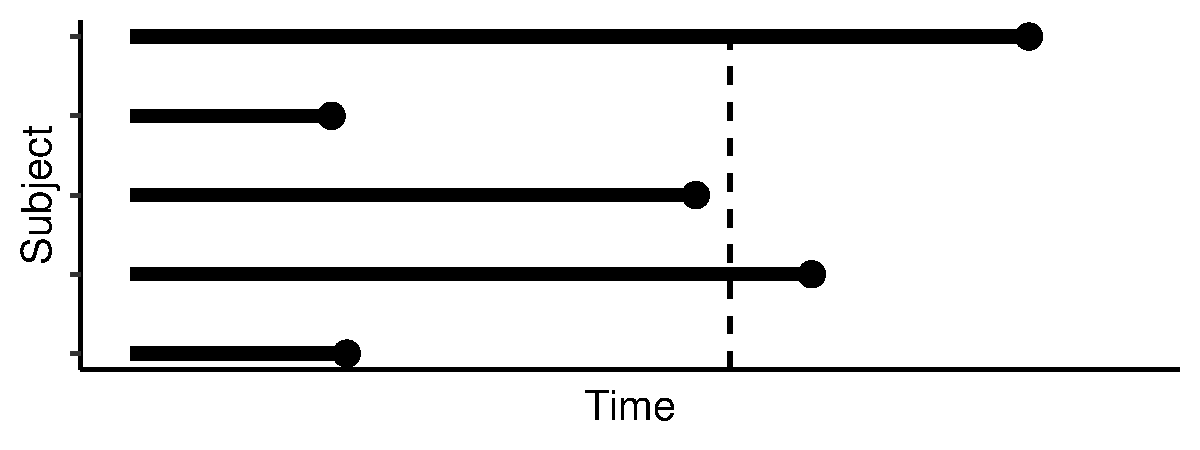
\includegraphics[width=\textwidth]{./fig-full-data.pdf}}
\end{picture}
\end{frame}

\begin{frame}[label={sec:org0128ddc}]{Risk prediction model and censored data}
\begin{picture}(320,250)
  \put(0,225){\begin{minipage}[t]{\linewidth} { For a fixed time horizon $t \in \R_+$ we have
\begin{description}
\item[{\(X \in \R^p\)}] Static covariates measured at baseline (\(t=0\))
\item[{\(\tilde T \in \R_+\)}] Observation time (\(\tilde T := T \wedge C\))
\item[{\(\Delta \in \{0,1\}\)}] Event indicator (\(\Delta := \1\{\tilde T = T\}\))
\item[{\(r(t \mid X) \in [0,1]\)}] Risk prediction at time \(t\) given baseline covariates
\item[{\(Y(t) \in \{0,1\}\)}] Is unobserved for som subjects
\end{description}
      }
    \end{minipage}}
  \put(0,20){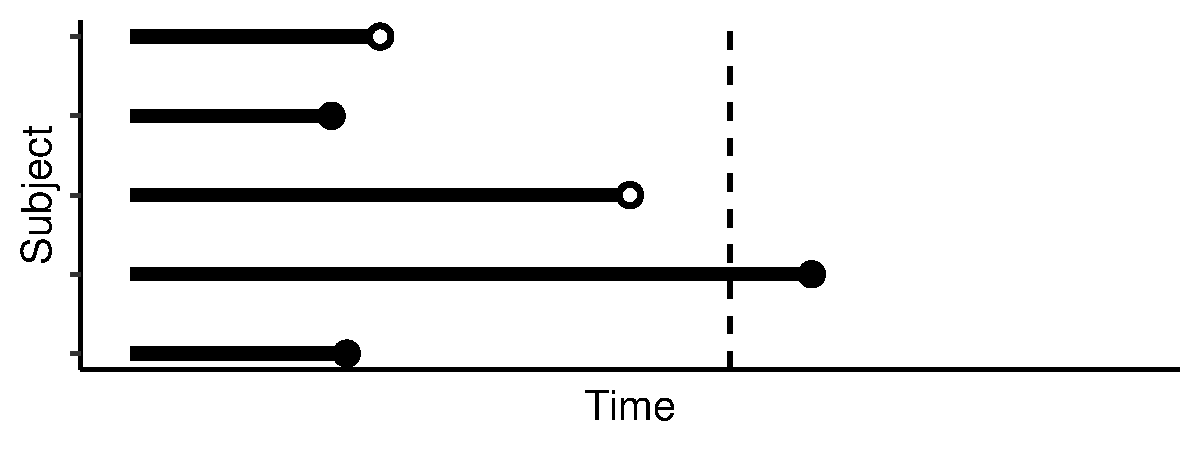
\includegraphics[width=\textwidth]{./fig-observed-data.pdf}}
\end{picture}
\end{frame}


\begin{frame}[label={sec:orgaca5d14}]{The Brier score}
Given a (non-random) risk-prediction model \(r \colon \R_+ \times \R^p \rightarrow [0,1]\) we want
to evaluate the performance of \(r\) at a fixed time horizon \(t \in \R_+\). For this we use the
Brier score
\begin{equation*}
  \E\left[ 
    \left\{
      Y(t) - r(t \mid X)
    \right\}^2 \right],
  \quad \text{with} \quad Y(t):= \1\{T \leq t\}.     
\end{equation*}

\begin{block}{Inverse probability of censoring weights (IPCW)}
Let $(X, T) \sim Q$ and $(X, \tilde T, \Delta) \sim P$. When $T \independent C \mid X$ the
Brier score is identifiable from the observed data\footnote<1->{Note that
  $W(t)\{Y(t)-r(t\mid X)\}^2$ is a function of the observed data, as $Y(t)$ is observed whenever
  $W(t)$ is non-zero.}:
\begin{equation*}
  \E_Q\left[ 
    \left\{
      Y(t) - r(t \mid X)
    \right\}^2 \right]
  = \E_P\left[
    W(t)
    \left\{
      Y(t) - r(t \mid X)
    \right\}^2 \right],
\end{equation*}
with
\begin{equation*}
  W(t) = \frac{\1({\tilde{T} >t})}{G(t \mid X)} + \frac{\1({\tilde{T}\leq
      t})\Delta}{G(\tilde{T}\mid X)},
\end{equation*}
and where $G(s \mid x) = P(C > s \mid X=x)$.
\end{block}
\end{frame}


\begin{frame}[label={sec:org2acd925}]{Visualizing the re-weighting}
\begin{equation*}
  \E_Q{\left[ 
    \left\{
      Y(t) - r(t \mid X)
    \right\}^2 \right]}
  = \E_P{\left[
    W(t)
    \left\{
      Y(t) - r(t \mid X)
    \right\}^2 \right]}
\end{equation*}    

\vfill

\begin{onlyenv}<1>
\begin{center}
\includegraphics[width=.9\linewidth]{/tmp/babel-CTEOPz/figure-04B68b.pdf}
\end{center}
\end{onlyenv}


\begin{onlyenv}<2>
\begin{center}
\includegraphics[width=.9\linewidth]{/tmp/babel-CTEOPz/figure-qxPs4l.pdf}
\end{center}
\end{onlyenv}


\begin{onlyenv}<3>
\begin{center}
\includegraphics[width=.9\linewidth]{/tmp/babel-CTEOPz/figure-QodefG.pdf}
\end{center}
\end{onlyenv}
\end{frame}


\begin{frame}[label={sec:org7dda4f6}]{Non-parametric estimation}
By estimating the censoring distribution \(G\) we obtain the IPCW estimator
\begin{equation*}
  \widehat{W}_i(t)=\frac{\1({\tilde{T}_i >t})}{\hat{G}(t \mid X_i)} + \frac{\1({\tilde{T}_i\leq
      t})\Delta_i}{\hat{G}(\tilde{T}_i\mid X_i)},
  \quad \hat{\theta}_n^t = \empmeas[\widehat{W}_i(t)
  \left\{
    Y_i(t) - r(t \mid X_i)
  \right\}^2]
\end{equation*}

\begin{block}{Inference and efficiency under non-parametric assumptions}
\begin{itemize}
\item Existing methods use Kaplan-Meier or Cox models to estimate the censoring distribution.
\item Non-parametric, data-adaptive estimation of the censoring distribution + inference
\(\rightarrow\) one-step estimators / DML / TMLE.
\end{itemize}
\end{block}

\begin{block}{Data-adaptive selection of the estimator \(\hat{G}\)}
Use some kind of cross-validation to select the best \(\hat{G}\) from a collection of candidates.
\pause \alert{Is it obvious how to do this?}
\end{block}
\end{frame}

\begin{frame}[label={sec:orgf62cea5}]{Cross validation for survival models -- the Brier score?}
\center \Large Brier score! \alt<4>{... infinite regress ...}{\color{white}{... infinite regress ...}}

\vfill


\begin{onlyenv}<2>
\begin{center}
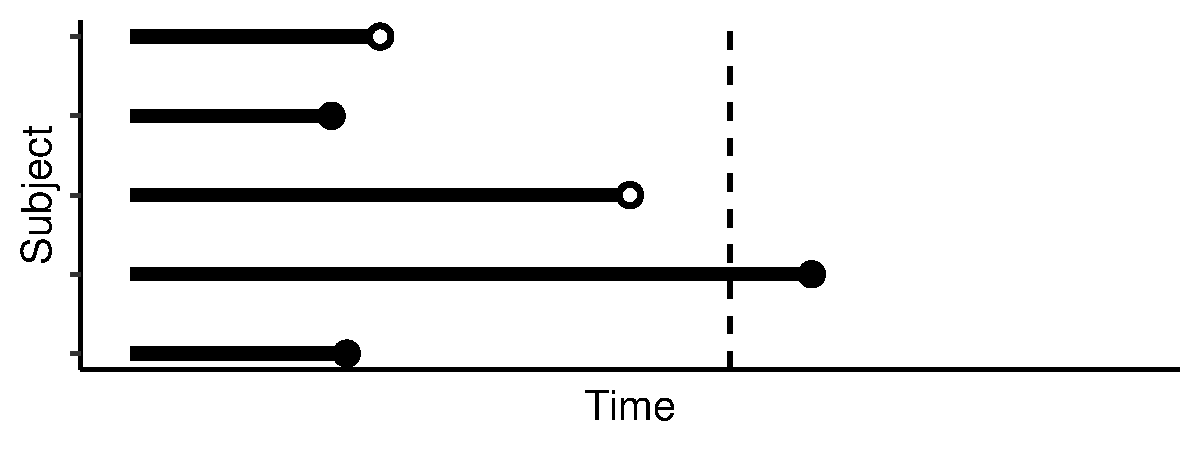
\includegraphics[width=.9\linewidth]{./fig-observed-data.pdf}
\end{center}
\end{onlyenv}

\begin{onlyenv}<3->
\begin{center}
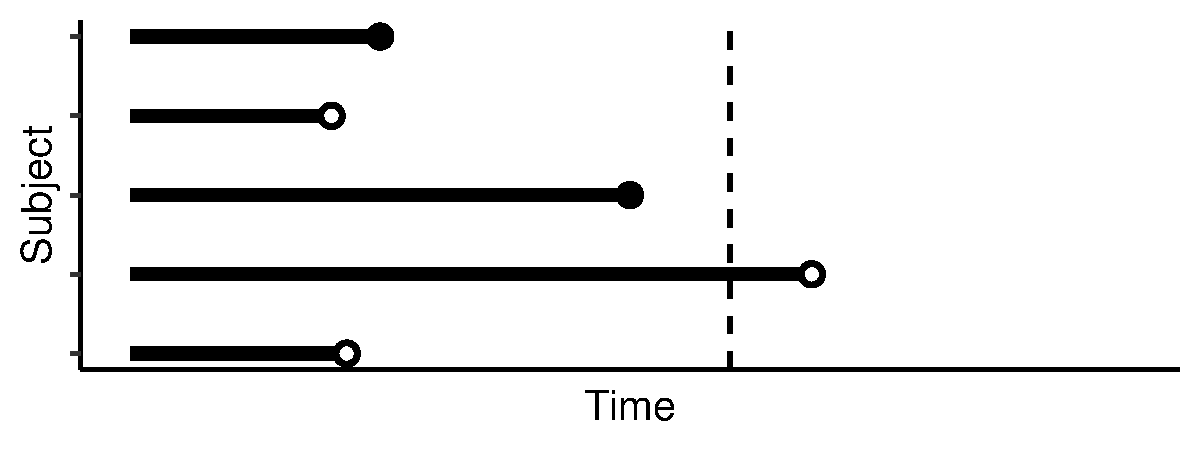
\includegraphics[width=.9\linewidth]{./fig-inverse-data.pdf}
\end{center}
\end{onlyenv}
\end{frame}


\begin{frame}[label={sec:org8205d06}]{Cross validation for survival models -- the likelihood?}
Many common estimators of a survival function will be a discrete measure \(\rightarrow\) the
likelihood will (a.s.) be 0 on any hold-out data sample.

\begin{onlyenv}<1>
\begin{center}
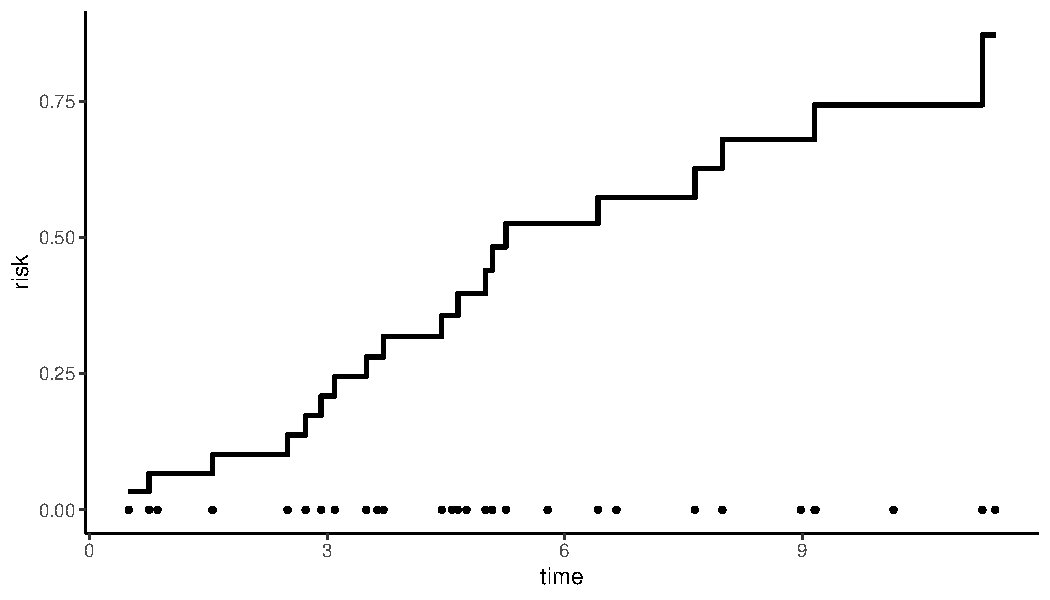
\includegraphics[width=.9\linewidth]{./km-plot.pdf}
\end{center}
\end{onlyenv}

\begin{onlyenv}<2->
\begin{center}
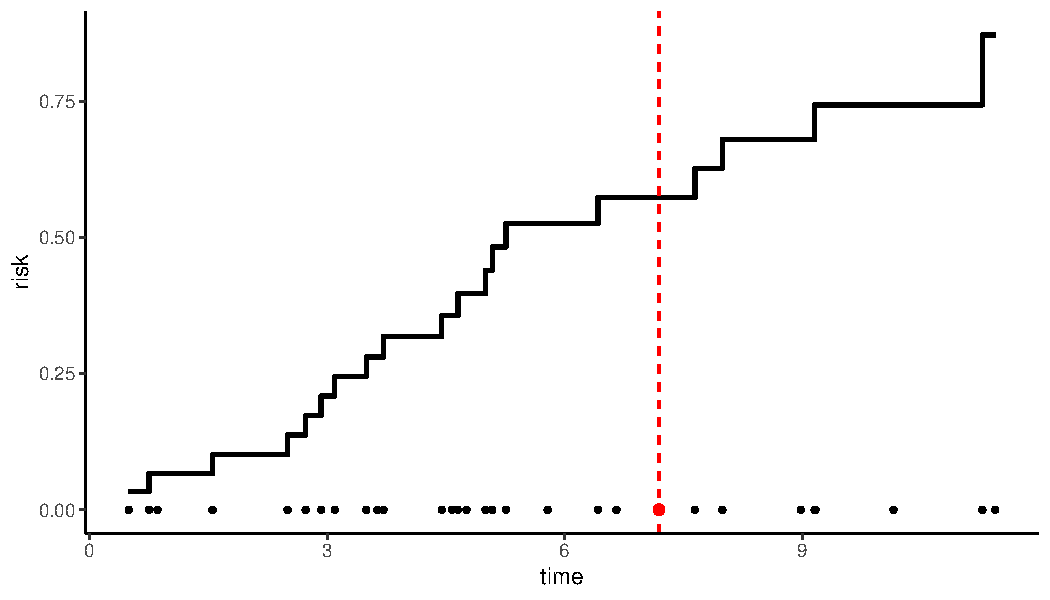
\includegraphics[width=.9\linewidth]{./km-plot-new-point.pdf}
\end{center}
\end{onlyenv}
\end{frame}

\begin{frame}[label={sec:org707419d}]{Summary}
\begin{beamercolorbox}[rounded=true]{gray}
\centering How should we do cross validation for general survival models when the
test and train data are censored?
\end{beamercolorbox}


\vfill

\begin{itemize}
\item Which other loss functions are sensible to use instead?
\item How can these (and the risk of an estimator) be approximated with observed data?

\vfill
\end{itemize}


\begin{block}{Questions, comments, suggestions?}
\vfill 

\flushright Thank you for listening!
\end{block}
\end{frame}

\section{References}
\label{sec:org1a91b15}
\tiny \bibliography{/home/amnudn/Documents/latex/default-bib.bib}
\end{document}